\documentclass[]{article}

\usepackage[a4paper, margin=25mm]{geometry}
\usepackage{graphicx}

\newcommand{\name}{DTI-Voodoo}

%opening
\title{\name{}: Supplement data}
\author{Tilman Hinnerichs and Robert Hoehndorf}
\date{}


\begin{document}

\maketitle

\begin{figure}[ht]%figure1
 	\centerline{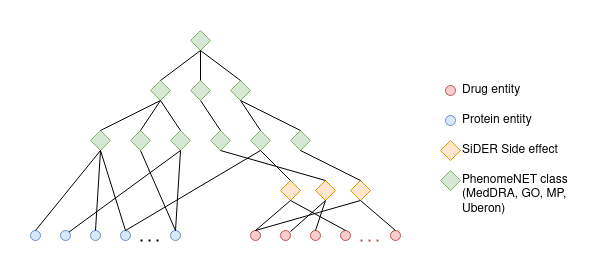
\includegraphics[width=0.9\textwidth]{../figures/drug_protein_ontology_network.png}}
 	\caption{Drugs and proteins with annotations to SiDER and PhenomeNET}
 	\label{fig:Onto}
\end{figure}

\begin{figure}[ht]%figure1
 	\centerline{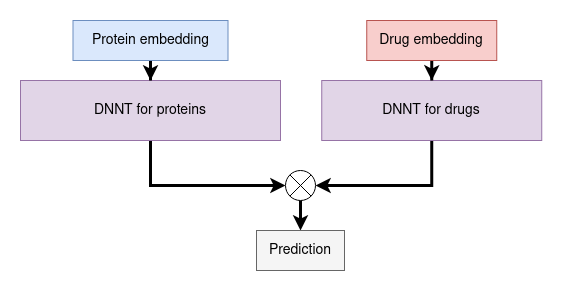
\includegraphics[width=0.75\textwidth]{../figures/siamese_network.png}}
 	\caption{Half-twin network applied to molecular and DL2vec
        features, utilizing deep learnable feature transformations
        (LFT). The similarity function $\otimes$ yields the
        similarity between both transformed embeddings e.g. by
        computing the cosine similarity.}
 	\label{fig:HalfTwinNetwork}
\end{figure}

\begin{figure}[ht]%figure1
 	\centerline{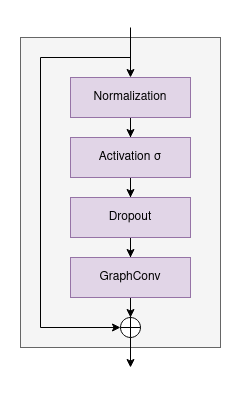
\includegraphics[width=0.3\textwidth]{../figures/ResGraphConvBlocks.png}}
 	\caption{Residual architecture built by \textit{Li et al. (2019, 2020b)} enabling deeper graph convolutional models}
 	\label{fig:ResGraphConvBlocks}
\end{figure}

\begin{figure}[ht]%figure1
	\centerline{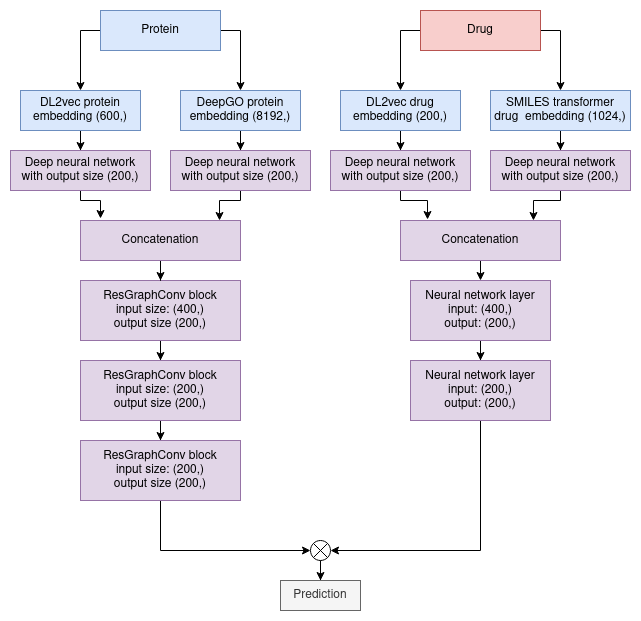
\includegraphics[width=1\columnwidth]{../figures/full_model_all_layers.png}}
	\caption{Residual architecture built by \textit{Li et al. (2019, 2020b)} enabling deeper graph convolutional models}
	\label{fig:FullModelAllLayers}
\end{figure}

\begin{table}[ht]
	\centering

	\begin{tabular}{|p{2.0cm}|p{1.1cm}|p{1.2cm}|p{0.8cm}|p{0.8cm}|p{1.2cm}|p{1.2cm}|}
		\hline
		Approach&\multicolumn{6}{c|}{Graph convolution method}\\
		&without&without/ empty RGC&GCN-Conv&GEN-Conv&RGC + GCNConv&RGC + GENConv\\
		\hline
		MolPred & $0.69$ & $0.67$& $0.67$& $0.68$& $0.65$& $0.69$\\
		\hline
		OntoPred &$0.88$ &$0.87$ &$0.88$&$0.90$&$0.86$&$0.92$\\
		\hline
		\name& $0.89$&$0.89$& $0.89$& $0.91$& $0.86$& $\mathbf{0.93}$\\
		\hline
	\end{tabular}
	\caption{\label{tab:Results}Results for various neural graph convolutional methods enhancing MolPred, OntoPred and \name{} over the STITCH dataset. We evaluated all methods over different stacking heights without and with residual graph convolution blocks (RGC, ResGraphConv) as depicted in Supplementary figure \ref{fig:ResGraphConvBlocks}. ``Empty RGC`` denotes a RGC block with a plain neural layer substituting the GraphConv layer.}
\end{table}


\begin{table}[ht]
	\centering
	\begin{tabular}{|p{2.0cm}|p{0.8cm}|p{0.8cm}|p{0.8cm}|p{0.8cm}|p{0.8cm}|p{0.8cm}|}
		\hline
		&\multicolumn{6}{c|}{(a) STITCH results}\\
		\hline
		\name{} results&\multicolumn{6}{c|}{PPI graph}\\
		&\multicolumn{3}{c|}{without}&\multicolumn{3}{c|}{with}\\
		&Macro AUC&Micro $AUC'_p$&Micro $AUC_p$&Macro AUC&Micro $AUC'_p$&Micro $AUC_p$\\
		\hline
		MolPred&$0.69$&$0.66$&$0.65$&$0.69$&$0.68$&$0.67$\\
		\hline
		OntoPred&$0.88$&$0.89$&$0.87$&$0.92$&$0.94$&$0.93$\\
		\hline
		\name{} & $0.89$& $0.91$ & $0.90$&$\mathbf{0.93}$&$\mathbf{0.94}$&$\mathbf{0.94}$\\
		\hline
	\end{tabular}
	\caption{Extended results table for MolPred, OntoPred and \name{} over STITCH with added $MicroAUC'_p$ for comparison of both metrics.}
\end{table}


\end{document}
